%% Article de participation EvalLLM 2026 -- equipe acss-psl
%% Modele CORIA-TALN-RJC 2026
\documentclass[10pt,twoside]{article}

\usepackage{times}
\usepackage[utf8]{inputenc}
\usepackage[T1]{fontenc}
\usepackage{graphicx}
\usepackage{booktabs}
\usepackage{array}
\usepackage{float}
\usepackage{placeins}
\usepackage{multirow}
\usepackage{tikz}
\usetikzlibrary{shapes.geometric, arrows.meta, positioning, fit, backgrounds}

\usepackage{siunitx}
\sisetup{locale = FR}

\usepackage{hyperref}
\usepackage{coria-taln2026}
\usepackage[french]{babel}

% Numéroter les sous-sections (2.1, 2.2, ...) et sous-sous-sections
\setcounter{secnumdepth}{3}

% Couleurs pour la figure pipeline
\definecolor{panelgray}{HTML}{F2F2F2}
\definecolor{panelamber}{HTML}{FFF7E6}
\definecolor{drawamber}{HTML}{D97706}
\definecolor{panelblue}{HTML}{EEF2FF}
\definecolor{drawblue}{HTML}{4F46E5}
\definecolor{panelgreen}{HTML}{E6F4EA}
\definecolor{drawgreen}{HTML}{137333}
\definecolor{numgreen}{HTML}{2D6A4F}

% Titre complet
\title{La liste de candidats comme goulot : liage d'entités de santé sans entraînement}

\author{Olivier Caron\\
  {\small
    DRM, Université Paris-Dauphine, Université PSL, CNRS, 75016 Paris, France \\
    \texttt{olivier.caron@dauphine.psl.eu} \\
}}

\begin{document}
\maketitle

% Contribution originale : la ligne \acceptedArticle reste commentee.
% \acceptedArticle[consignes]{}{}

\resume{
  Nous décrivons le système de l'équipe ACSS-PSL pour la tâche de liage d'entités du défi
  EvalLLM~2026~: relier chaque mention de santé pré-identifiée à un identifiant GeoNames (lieux)
  ou MeSH (pathogènes, maladies, toxines), ou la marquer comme hors-référentiel. Notre approche
  est frugale et sans entraînement. Une cascade de règles déterministes (normalisation, détection
  des cas hors-référentiel, génération de candidats par index local) est suivie d'un grand modèle
  de langue (LLM), appelé seulement sur les cas ambigus. Ce modèle choisit dans une liste fermée et ne
  génère jamais d'identifiant. Sur le jeu d'entraînement, le même score (RANKING 92,22) est obtenu
  que le modèle soit l'API GPT-5.4-nano ou un modèle ouvert local (gemma-4-31b, Qwen3.6-35B-A3B).
  Ce plateau partagé suggère que le goulot n'est pas le LLM mais la liste de
  candidats. L'empreinte carbone du run local est mesurée à environ 1,15~g équivalent
  CO\textsubscript{2}.
}

\abstract{\NoAutoSpaceBeforeFDP{}The Candidate List as the Bottleneck: Training-Free Health Entity Linking}{
  We describe the ACSS-PSL system for the entity linking task of the EvalLLM~2026 challenge:
  linking each pre-identified health mention to its identifier (GeoNames for places, MeSH for
  pathogens, diseases and toxins), or marking it as out-of-knowledge-base. Our approach is
  frugal and training-free. A deterministic cascade of rules (normalisation, out-of-base
  detection, candidate generation from local indexes) is followed by an LLM used only to
  disambiguate the remaining ambiguous cases. On the training set, the same score
  (RANKING 92.22) is reached whether the model is the GPT-5.4-nano API or an open model served
  locally (gemma-4-31b, Qwen3.6-35B-A3B), which suggests the bottleneck is the candidate list, not
  the LLM. The carbon
  footprint of the local run is measured at about 1.15~g CO\textsubscript{2}-equivalent.
}

\motsClefs
  {liage d'entités, génération de candidats, GeoNames, MeSH, LLM, veille sanitaire}
  {entity linking, candidate generation, GeoNames, MeSH, LLM, health surveillance}

%%================================================================
\section{Introduction}
\label{sec:intro}

La veille sanitaire repose en partie sur la lecture de textes en français (dépêches, rapports,
articles) où il faut identifier des lieux et des agents de santé, puis les relier à des
référentiels stables. Le défi EvalLLM~2026 propose cette tâche de \emph{liage d'entités}~:
les mentions sont déjà repérées dans le texte, et il faut associer à chacune un identifiant
dans GeoNames pour les lieux, ou dans MeSH pour les pathogènes, maladies et toxines, ou bien
décider qu'aucune entrée du référentiel ne convient (cas hors-référentiel, ou NIL).

Le cadre est celui des très faibles ressources~: le jeu d'entraînement ne contient que
quelques dizaines de documents annotés. Entraîner un modèle génératif dans ces conditions
exposerait à un fort risque de surapprentissage. Nous faisons donc le choix inverse, frugal~:
aucun modèle n'est entraîné. Le cœur du système est une cascade de règles
déterministes qui s'appuie sur des index locaux (GeoNames, MeSH). Un grand modèle de
langue (\emph{Large Language Model}, LLM) n'intervient qu'en dernier recours, pour départager les seuls cas où plusieurs
candidats subsistent.

Ce choix soulève une question simple~: le LLM est-il le facteur limitant~? Nous montrons que non.
En remplaçant le modèle de désambiguïsation par trois modèles très différents (une API
propriétaire et deux modèles ouverts), nous obtenons le même score sur le jeu d'entraînement. Le
goulot se situe ailleurs, dans la couverture de la liste de candidats. Plusieurs ablations
l'étayent (section~\ref{sec:resultats}). Par souci de transparence, nous soumettons une
configuration enrichie de quelques règles issues du fichier de test et une configuration
strictement généraliste, sans effet sur le score d'entraînement. L'empreinte carbone est mesurée
pour le run local (Green Algorithms) et estimée pour l'API (EcoLogits). Le code est disponible
publiquement\footnote{\url{https://github.com/oliviercaron/acss-psl-evalllm2026}.}.

%%================================================================
\section{Travaux connexes}
\label{sec:related}

\subsection{Liage d'entités biomédicales}
Le liage d'entités biomédicales s'appuie souvent sur un pré-entraînement coûteux, qu'il
repose sur des représentations denses
(BioSyn~\cite{sung2020biosyn}, SapBERT~\cite{liu2021sapbert}, KRISSBERT~\cite{zhang2022krissbert},
ou les représentations de BioLORD-2023~\cite{remy2023biolord} dont le liage est l'une des tâches
d'évaluation) ou sur la génération
(GenBioEL~\cite{yuan2022genbioel}). L'évaluation comparative de \shortcite{kartchner2023bioel}
décrit le cadre en deux étapes, une génération de candidats peu coûteuse suivie d'une
désambiguïsation plus précise, et rappelle que les grands modèles génératifs hallucinent. Pour le
français, les ressources biomédicales restent limitées, en particulier pour la normalisation
d'entités~: \shortcite{wajsburt2021normalization} rapportent que moins de 4\,\% des concepts de
l'UMLS disposent d'un terme français. Plus largement, les travaux récents sur le TAL biomédical
français, tels que DrBERT~\cite{labrak2023drbert} et
CamemBERT-bio~\cite{touchent2023camembertbio}, illustrent que l'adaptation au domaine repose sur un
pré-entraînement dédié, même lorsque l'évaluation porte sur d'autres tâches de TAL biomédical (reconnaissance d'entités,
classification, questions-réponses) plutôt que sur le liage. Pour pallier cette rareté, xMEN~\cite{borchert2025xmen} génère des candidats
multilingues en exploitant les alias anglais quand ceux de la langue cible manquent.

\subsection{Modèles de langue comme désambiguïsateurs contraints}
Plusieurs travaux récents emploient un modèle de langue à l'étape de désambiguïsation d'un liage en
deux temps, sans entraînement. \shortcite{ye2025disambiguator} montrent qu'un modèle de langue
utilisé comme désambiguïsateur sur des listes de candidats biomédicaux améliore nettement l'exactitude
sans fine-tuning, et que la performance dépend fortement de la qualité de la génération de
candidats. Pour empêcher le modèle de produire des identifiants invalides,
\shortcite{lin2025llm4bioel} contraignent son décodage au niveau des jetons aux entités valides de
la base. Le cas où le bon candidat est absent de la liste est un
problème reconnu du reranking~: \shortcite{zhou2024gendecider} montrent que supposer le bon candidat
toujours présent ne tient pas en contexte zero-shot, et qu'un jugement explicite d'absence renseigne
sur les limites de la génération de candidats.

LELA~\cite{haffoudhi2026lela} propose une chaîne sans entraînement qui génère des candidats puis
laisse un modèle de langue choisir l'entité finale par son indice dans une liste fermée, avec un
modèle à raisonnement et auto-cohérence. LELA cible la généralisation zero-shot sur des bancs d'essai anglophones variés (Wikipedia, acronymes,
compétences professionnelles).

%%================================================================
\FloatBarrier
\section{Tâche et données}
\label{sec:tache}

Pour chaque mention pré-annotée (texte, type, position), il faut produire un identifiant et sa
source~: GeoNames pour les lieux (type \textsc{location}), MeSH pour les pathogènes, maladies et
toxines, ou une absence d'identifiant pour les cas hors-référentiel. Le jeu d'entraînement
compte 40 documents et 491 entités annotées (dont 470 avec identifiant de référence et 21
hors-référentiel), et le jeu de test 200 documents et 1840 entités sans référence fournie aux
participants. Le guide d'alignement fourni par l'organisation
précise les conventions de liage, et nous nous y conformons. Le classement officiel, que nous
notons RANKING, est la moyenne de deux métriques fournies par l'organisation~: l'exactitude InKB
partielle (crédit partiel sur les concepts quand les descripteurs principaux sont corrects), qui
évalue la désambiguïsation sur les seules mentions liables (NIL exclus), et la
F-mesure de liage (\emph{NEL F1}), qui évalue le système complet (NIL compris). Nous rapportons les
scores officiels sur le test (section~\ref{sec:resultats}). Les analyses fines de réglage et
d'erreurs s'appuient sur le jeu d'entraînement, faute d'annotation de référence sur le test.

La difficulté de liage n'est pas la même selon le référentiel. La
figure~\ref{fig:ambiguite} montre, pour les 470 entités à lier du corpus (hors 21 NIL), le nombre de
candidats que l'index retrouve avant désambiguïsation. Côté MeSH, le dictionnaire résout
presque toujours la mention à un seul concept, si bien que le LLM n'est quasiment jamais sollicité. Côté GeoNames, au
contraire, la majorité des lieux donne lieu à plusieurs candidats homonymes
(2 à 5, 6 à 20, voire plus de 20), ce qui rend la désambiguïsation indispensable. C'est donc
sur les lieux que se concentre le travail du LLM.

\begin{figure}[!htb]
\centering
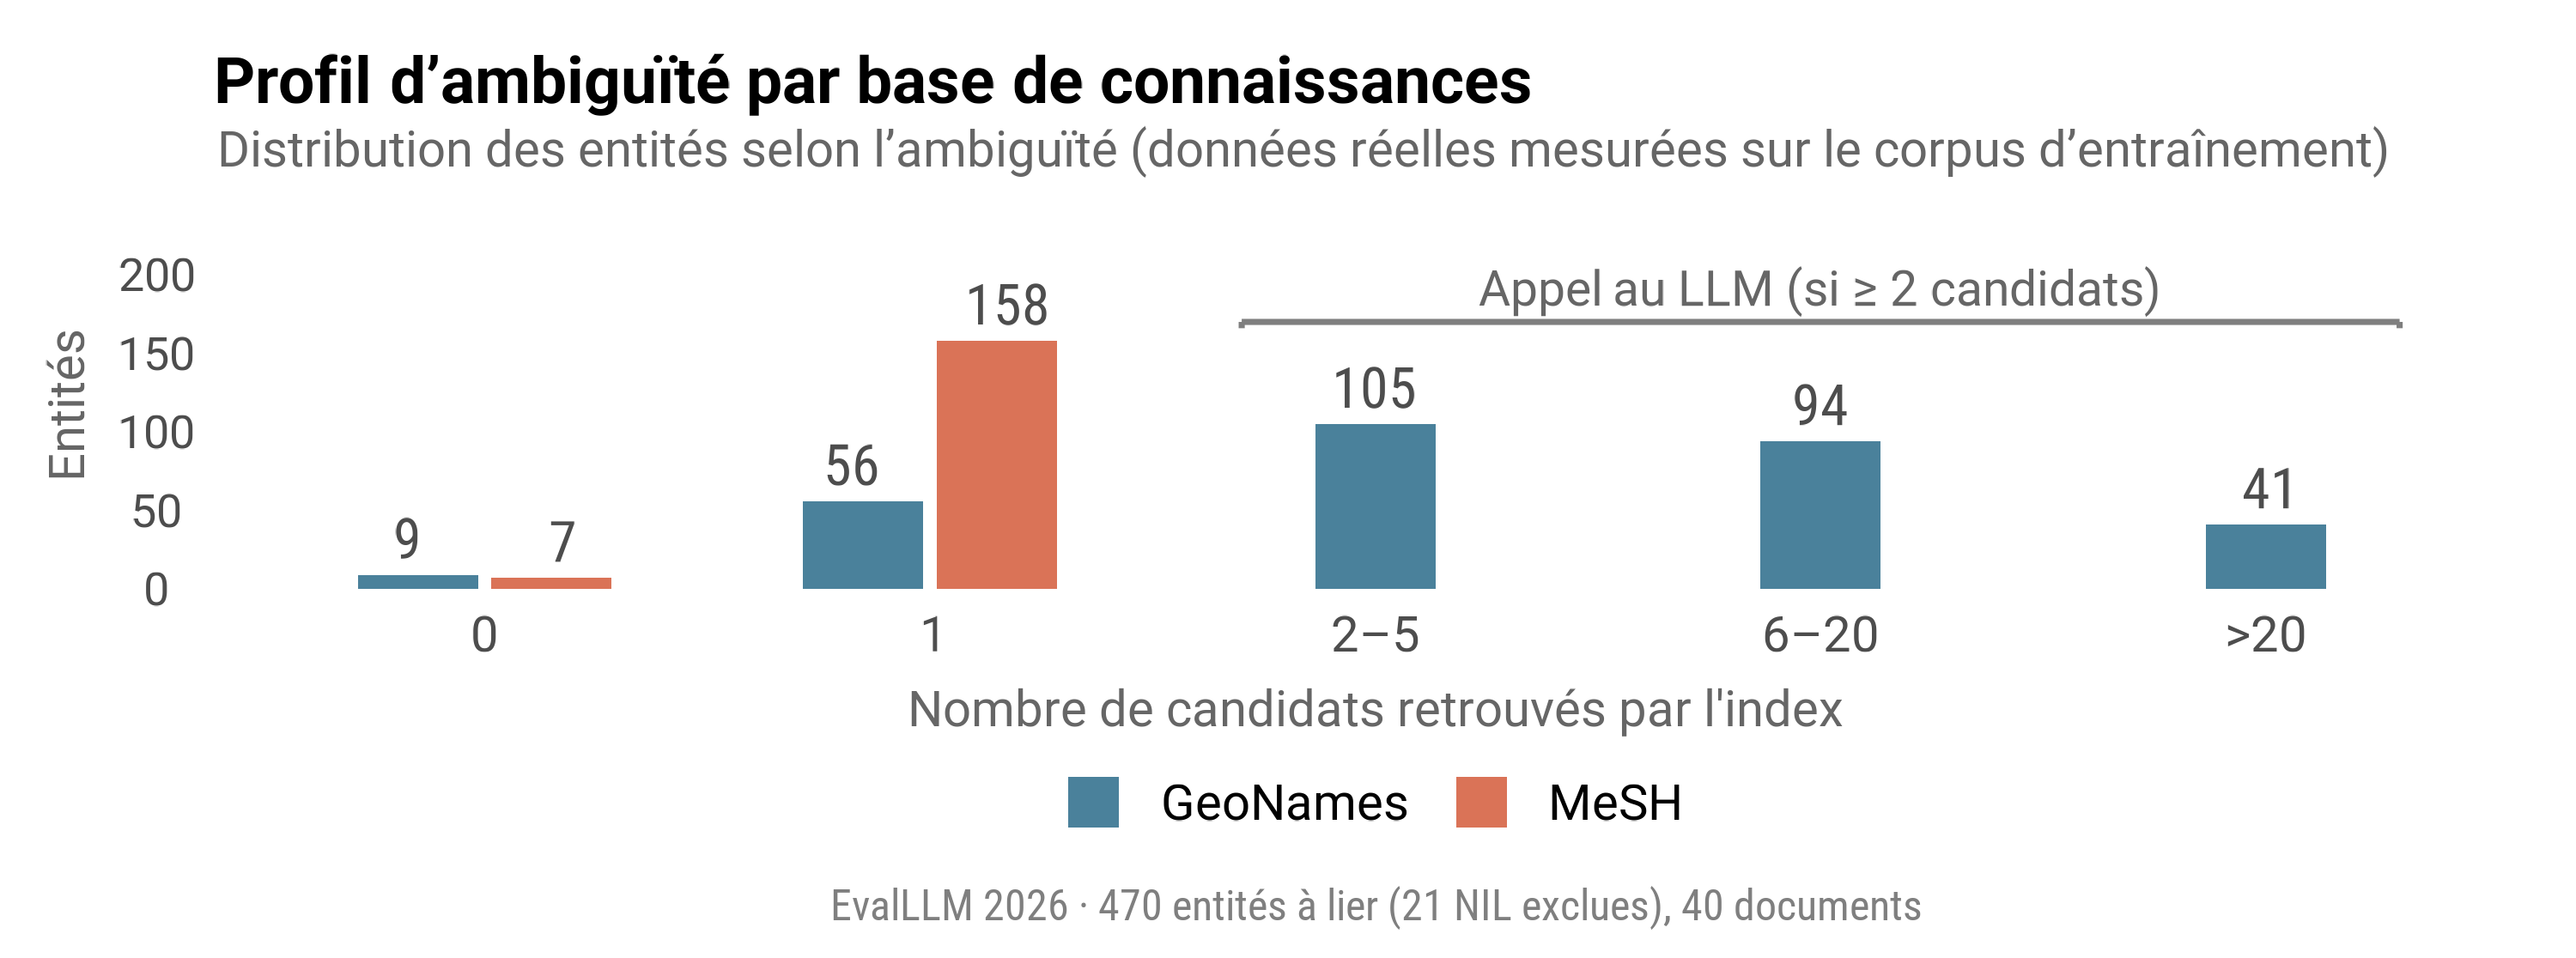
\includegraphics[width=0.82\textwidth]{fig_ambiguity_profile.png}
\caption{Profil d'ambiguïté par référentiel sur le corpus d'entraînement~: distribution des
470 entités à lier (les 21 NIL exclues) selon le nombre de candidats retrouvés par l'index avant
désambiguïsation.}
\label{fig:ambiguite}
\end{figure}

%%================================================================
\FloatBarrier
\section{Système}
\label{sec:systeme}

Le système traite chaque mention par une cascade déterministe. Le LLM n'intervient qu'à la fin, et seulement si plusieurs candidats subsistent
(figure~\ref{fig:pipeline}).

\begin{figure}[!t]
\centering
\scalebox{0.92}{%
\begin{tikzpicture}[
  node distance=2.5mm,
  % numbered circle for step labels
  num/.style={circle, fill=#1, text=white, font=\sffamily\bfseries\scriptsize,
              inner sep=0pt, minimum size=4mm},
  % main boxes
  panel/.style 2 args={draw=#2, rounded corners=3pt, fill=#1,
                text width=105mm, align=left, inner sep=2mm, font=\footnotesize},
  panelgr/.style={draw=gray!60, rounded corners=3pt, fill=panelgray,
                text width=105mm, align=left, inner sep=2mm, font=\footnotesize},
  % narrow side box
  sidebox/.style={draw=red!60, rounded corners=3pt, fill=red!8,
                  align=center, font=\footnotesize\sffamily, inner sep=2mm},
  % arrows
  arr/.style={-{Stealth[length=2mm]}, gray!70, thick},
  dotarr/.style={-{Stealth[length=2mm]}, gray!50, thick, densely dotted},
]

% ── 1. ENTRÉE + NORMALISATION ────────────────────
\node[panelgr] (innorm) {%
  \textsf{\textbf{ENTRÉE + NORMALISATION}}\\[0.5pt]
  Le fournisseur de ces graines était la société britannique Thompson \& Morgan, basée à
  \tikz[baseline=(X.base)]{\node[fill=orange!25, rounded corners=2pt,
    inner sep=1.5pt] (X) {\textbf{Ipswich}};}.\\[0.5pt]
  {\scriptsize mention pré-identifiée~: \textbf{Ipswich} (type \textsc{location})
  \enspace$\rightarrow$\enspace \texttt{ipswich} \enspace$\cdot$\enspace dans le référentiel, on continue}
};
\node[num=gray!55, anchor=south east] at ([shift={(-0.5mm,0.5mm)}]innorm.north west) {1};

% ── branche NIL ────────────────────────────────────────────
\node[sidebox, right=12mm of innorm] (nil) {\textbf{NIL}\\(non liée)};
\draw[dotarr] (innorm.east) -- node[above, font=\scriptsize\itshape, text=gray]{sinon} (nil.west);

% ── 2. GÉNÉRATION DE CANDIDATS ─────────────────────────────
\node[panelgr, below=of innorm] (cg) {%
  \textsf{\textbf{GÉNÉRATION DE CANDIDATS}} : index GeoNames local\\[0.5pt]
  requête \texttt{"ipswich"} (correspondance exacte) $\rightarrow$ 13 candidats, top-5 conservé
};
\node[num=gray!55, anchor=south east] at ([shift={(-0.5mm,0.5mm)}]cg.north west) {2};

% ── 3. CANDIDATS ───────────────────────────────────────────
\node[panel={panelamber}{drawamber}, below=of cg] (cand) {%
  \textsf{\textbf{CANDIDATS}}\\[1pt]
  {\scriptsize\ttfamily
  \begin{tabular}[t]{@{}l@{}}
  {[0]} Ipswich, Australie, pop.\ 229\,208, id 7839586\\
  {[1]} Ipswich, Royaume-Uni, pop.\ 178\,835, id 2646057\\
  {[2]} Ipswich, États-Unis, pop.\ 959, id 5228742\\
  {[3]} New Ipswich, États-Unis, pop.\ 5\,194, id 5090188\\
  {[4]} Ipswich, États-Unis, pop.\ 4\,222, id 4940625
  \end{tabular}}
};
\node[num=drawamber, anchor=south east] at ([shift={(-0.5mm,0.5mm)}]cand.north west) {3};

% ── 4. PROMPT ──────────────────────────────────────────────
\node[panel={panelblue}{drawblue}, below=of cand] (prompt) {%
  \textsf{\textbf{Prompt (anglais, température 0)}}\\[1pt]
  {\scriptsize\ttfamily
  You select the GeoNames entry that matches a place\\
  mentioned in a French news article.\\
  CONTEXT: "...la société britannique Thompson \& Morgan,\\
  \hspace*{2.5em}basée à Ipswich."\\
  MENTION: "Ipswich" \enspace CANDIDATES: [0]\ldots[4]\\
  Reply with ONLY the candidate number (0-4).}
};
\node[num=drawblue, anchor=south east] at ([shift={(-0.5mm,0.5mm)}]prompt.north west) {4};

% ── 5. MODÈLE + RÉPONSE ────────────────────
\node[panel={panelgreen}{drawgreen}, below=of prompt] (llmout) {%
  \textsf{\textbf{MODÈLE DE LANGUE}} {\footnotesize(choix dans la liste)}\\[1pt]
  réponse~:
  \tikz[baseline=(R.base)]{\node[draw=gray!50, rounded corners=2pt,
    fill=white, inner sep=1.5pt, font=\ttfamily\bfseries\footnotesize] (R) {1};}
  \enspace{\scriptsize\itshape « société britannique » $\Rightarrow$ Royaume-Uni}\\[1pt]
  \textsf{\textbf{RÉPONSE FINALE}}\enspace$\longrightarrow$ \textbf{GeoNames 2646057} {\scriptsize(Ipswich, R.-U.)}
};
\node[num=numgreen, anchor=south east] at ([shift={(-0.5mm,0.5mm)}]llmout.north west) {5};

% ── FLÈCHES PRINCIPALES ─────────────────────────
\foreach \a/\b in {innorm/cg, cg/cand, cand/prompt, prompt/llmout} {
  \draw[arr] (\a.south) -- (\b.north);
}

\end{tikzpicture}%
}
\caption{Exemple réel de liage tiré du corpus d'entraînement (enquête sur une épidémie à E.~coli
liée à des graines de fenugrec). La mention « Ipswich », ambiguë entre treize homonymes, est résolue
vers le Royaume-Uni grâce à l'indice contextuel « société britannique ». Tous les candidats,
identifiants et populations sont ceux réellement produits par le programme.}
\label{fig:pipeline}
\end{figure}

La cascade commence par normaliser la mention~: passage en minuscules, nettoyage typographique,
variantes sans accents, et translittération du grec en dernier recours. Un filtre de motifs lexicaux
marque ensuite comme non liées les mentions manifestement absentes du référentiel (quartiers, zones,
bassins, ceintures, venins bruts). Les concepts
géographiques nus sont traités avec prudence~: lorsqu'une périphrase référentielle est reconnue
(par exemple « continent africain » ou « territoire américain »), elle est redirigée vers un
pays ou un continent par une règle dédiée, sinon la mention peut rester non liée selon le guide
d'alignement.

Le traitement diverge ensuite selon le référentiel. Pour les lieux, une première couche de règles
générales (validées sur le guide et le jeu d'entraînement) redirige certaines mentions vers leur entité
géographique~: « Hexagone » vers « France », une périphrase « territoire » suivie d'un gentilé vers
le pays, ou les sous-régions des Nations unies. Un index SQLite de GeoNames génère ensuite les
candidats, par plusieurs passes de correspondance sur les noms, les noms francisés et les codes de
type de lieu de GeoNames. Un post-traitement géographique tranche~: préférence au pays, à la capitale ou
au chef-lieu, réconciliation des codes par les coordonnées, et garde-fous contre les rues et
bâtiments. Pour les concepts biomédicaux, un dictionnaire français curé associe les termes
courants à leur descripteur MeSH, et des règles propres aux étiquettes séparent le pathogène de la
maladie (par exemple le virus du VIH et le SIDA). En cas d'échec, un index MeSH bilingue est
interrogé. S'y ajoutent une règle « souche » (par exemple \emph{E.~coli} O104) et une règle qui propage, dans
tout le document, le lien d'un acronyme vers sa forme développée.

Quand au moins deux candidats subsistent après ces étapes, un LLM choisit dans la liste complète
des candidats (\emph{listwise reranking}). C'est le seul appel au LLM, et il est volontairement
contraint. À température 0, le
modèle reçoit deux choses~: un extrait local de $\pm$200 caractères autour de la mention (borné à
500 caractères dans le prompt) et une liste numérotée de candidats. Il répond par un seul indice, et
l'identifiant final est lu dans la liste. Le modèle ne génère jamais d'identifiant, ce qui
rend les erreurs analysables comme un défaut de génération de candidats ou de choix dans la liste.
Nous limitons la liste à cinq candidats pour les lieux (réglage justifié en
section~\ref{sec:resultats}) et à dix pour les concepts, sans effet observé côté MeSH où l'index ne
renvoie quasiment jamais plus d'un candidat. Un extrait du prompt figure en annexe~\ref{ann:prompt}
et les hyperparamètres complets en annexe~\ref{ann:hyper}. Chaque règle ajoutée est verrouillée par
des tests de non-régression (104 tests~: détection NIL, périphrases, translittération du grec,
règle de souche, garde-fous contre les rues et bâtiments, validateur de format de soumission),
de sorte qu'un ajout n'invalide pas un cas déjà résolu.

%%================================================================
\section{Configuration expérimentale}
\label{sec:config}

Les trois runs varient selon deux axes~: le modèle de désambiguïsation et la présence de deux
ressources additionnelles (règles issues de l'examen du fichier de test, exonymes français
tirés de Wikidata). Le cache Wikidata n'est pas un référentiel de sortie~: il contient seulement,
pour quelques lieux restés NIL après la cascade GeoNames, des identifiants GeoNames récupérés
hors ligne via la propriété Wikidata P1566. À la prédiction, aucun accès réseau n'est effectué.
Ces identifiants sont rechargés depuis la base GeoNames locale, filtrés puis désambiguïsés comme
les autres candidats. Cette configuration généraliste (run~2) est dérivée du run~3 sans relancer le LLM~: les
ajouts issus de l'examen du test (cache d'exonymes Wikidata vers GeoNames, clusters Marburg,
encéphalite à tiques, VHC) sont ramenées à NIL par une règle déterministe
(tableau~\ref{tab:runs}). Pour l'étape de désambiguïsation,
nous comparons l'API GPT-5.4-nano (température 0) à des modèles ouverts servis localement avec
vLLM~\cite{vllm2023} sur un GPU NVIDIA H100~: gemma-4-31b (31~milliards de paramètres) et
Qwen3.6-35B-A3B (un modèle à mélange d'experts, raisonnement désactivé), ainsi que la famille
Qwen2.5 (7, 32 et 72~milliards) à titre de comparaison. Toutes les évaluations sur le jeu d'entraînement sont
conduites sans la mémoire d'entraînement (option \texttt{--no-memory}), de sorte que le score mesure
la cascade de règles et le modèle de langue, et non un rappel direct des annotations déjà vues.
L'énergie du GPU local est mesurée
directement par échantillonnage de la puissance (nvidia-smi à 1~Hz), puis convertie selon la
méthode Green Algorithms~\cite{lannelongue2021green}. Pour les appels d'API, dont le matériel
n'est pas observable, l'empreinte est estimée avec EcoLogits~\cite{ecologits}.

\begin{table}[!h]
\centering
\small
\setlength{\tabcolsep}{5pt}
\begin{tabular}{llll}
\toprule
Run & Modèle (étape 5) & Couverture & Liées / NIL \\
\midrule
run~1 & gemma-4-31b (local) & étendue & 1700 / 140 \\
run~2 & GPT-5.4-nano (API) & généraliste & 1654 / 186 \\
run~3 & GPT-5.4-nano (API) & étendue & 1700 / 140 \\
\bottomrule
\end{tabular}
\caption{Les trois runs soumis (jeu de test, 1840 mentions). La couverture « étendue » ajoute
quelques termes spécialisés et un cache d'exonymes Wikidata vers GeoNames. La version généraliste
retire ces ajouts par retour déterministe vers NIL, ce qui explique les 46 mentions de différence.}
\label{tab:runs}
\end{table}

Plusieurs alternatives plus lourdes ont été testées sur le jeu d'entraînement puis écartées faute de
gain. Sur la configuration à dix candidats, un prompt rédigé entièrement en français dégrade le RANKING
de 91,19 à 90,12, une perte portée uniquement par GeoNames (F1 89,84 contre 88,20), MeSH restant
inchangé car ses candidats sont présentés de façon bilingue. Ce résultat rejoint les travaux
montrant que les instructions anglaises surpassent souvent leur traduction pour les modèles
\emph{English-centric}~\cite{lai2023beyond}, un effet cohérent avec l'existence d'un espace conceptuel interne
biaisé vers l'anglais~\cite{wendler2024llamas}. Le liage d'entités y reste d'ailleurs peu
exploré~\cite{zaghir2024prompt}. Le vote majoritaire sur gemma n'apporte
pas de gain. Le réglage de la taille de liste est traité au
tableau~\ref{tab:listwise}.

%%================================================================
\section{Résultats}
\label{sec:resultats}

\subsection{Le LLM n'est pas le facteur limitant}
Le tableau~\ref{tab:plateau} donne le score d'entraînement pour chaque modèle de désambiguïsation.
Trois modèles très différents atteignent exactement le même RANKING de 92,22, avec les
mêmes F-mesures par référentiel (GeoNames et MeSH). Passer de 32 à 72~milliards de paramètres au sein
de la famille Qwen2.5 ne modifie pas le score (91,59). Dans les configurations testées sur le jeu d'entraînement, le score ne dépend
donc ni du modèle ni de sa taille au-delà d'un seuil, et la F-mesure MeSH est identique pour tous, les listes de candidats MeSH
étant courtes. Côté GeoNames, le LLM est pourtant sollicité sur 240 des 305 mentions (celles à au
moins deux candidats), et les trois modèles y atteignent la même F-mesure (91,06). Le fait que le choix du
modèle ne modifie pas le score sur la portion où il est le plus sollicité rejoint la section~\ref{subsec:goulot}~: le
résiduel d'erreurs tient à la génération de candidats (référence absente de la liste ou mauvais
niveau administratif), un problème qui s'impose à tout reranker.

\begin{table}[!h]
\centering
\small
\setlength{\tabcolsep}{4.5pt}
\begin{tabular}{lccccc}
\toprule
Modèle (étape 5) & RANKING & InKB part. & NEL F1 & F1 GeoNames & F1 MeSH \\
\midrule
GPT-5.4-nano (API) & \textbf{92,22} & 92,12 & 92,32 & 91,06 & 94,74 \\
gemma-4-31b (local) & \textbf{92,22} & 92,13 & 92,32 & 91,06 & 94,74 \\
Qwen3.6-35B-A3B (local) & \textbf{92,22} & 92,13 & 92,32 & 91,06 & 94,74 \\
\midrule
Qwen2.5-72B (local) & 91,59 & 91,49 & 91,68 & 90,08 & 94,74 \\
Qwen2.5-32B (local) & 91,59 & 91,49 & 91,68 & 90,08 & 94,74 \\
Qwen2.5-7B (local) & 87,33 & 87,23 & 87,42 & 83,58 & 94,74 \\
\bottomrule
\end{tabular}
\caption{Score d'entraînement selon le modèle de désambiguïsation. Le RANKING est la moyenne de
l'exactitude partielle InKB et de la F-mesure de liage (NEL F1). Les
valeurs affichées sont arrondies à deux décimales, le RANKING étant calculé sur les valeurs non
arrondies (d'où 92,22 malgré des InKB partielles de 92,12 et 92,13).}
\label{tab:plateau}
\end{table}

\subsection{Réglages de la désambiguïsation}
Nous avons isolé l'effet du nombre de candidats GeoNames en fixant le contexte à $\pm$200
caractères et en ne faisant varier que la taille de la liste (tableau~\ref{tab:listwise} en
annexe, deux exécutions par configuration). La liste courte est la plus efficace, et de façon stable~: le top-5
atteint 92,22 sur ses deux tirages (variance nulle), au-dessus de toute la bande de variance des
listes plus longues, qui forment un plateau bruité de dix à vingt candidats (91,8 à 91,9). Donner à la fois davantage de contexte ($\pm$600) et davantage de
candidats (top-30) n'apporte pas de gain (91,21 contre 91,42). Toutefois, ce test fait varier deux facteurs à la
fois, il ne prouve donc pas l'optimalité de 200 caractères, mais il montre que l'ajout naïf
d'information ne résout pas les cas difficiles. Avec deux tirages par configuration, ces écarts sont
un indice, non une preuve statistique.

\subsection{Le goulot est souvent la liste de candidats}
\label{subsec:goulot}
Nous avons inspecté les erreurs au moyen d'un visualiseur HTML autonome qui affiche, pour chaque
erreur, le document avec la mention surlignée, le lien attendu et le lien prédit. Pour les lieux,
il ajoute la liste des candidats GeoNames réellement générés avec le rang de la référence
(annexe~\ref{ann:erreurs}). Cette inspection montre que beaucoup d'erreurs GeoNames ne sont pas
des erreurs de choix mais de génération de candidats. Sur les vingt-quatre erreurs d'identifiant
GeoNames examinées, le bon identifiant est
absent de la liste dans six cas (par exemple « Caucase » ou « commune IV de Bamako ») et placé au-delà du
rang retenu dans deux autres (« Sedan » au rang 37). Dans ces situations, aucun reranker, même
plus grand, ne peut sélectionner un candidat qui n'a pas été produit. Les seize erreurs restantes
sont des confusions de niveau administratif, comme « Cannes » ou « Bègles » liés à la commune
plutôt qu'à la localité, ou « Amesbury », dont les métadonnées sont pauvres. Elles relèvent du choix du bon
code de \emph{feature} et du post-traitement géographique, pas du reranking sémantique.

\subsection{Résultats officiels sur le test}
Les scores officiels communiqués par l'organisation prolongent l'analyse tirée du jeu d'entraînement. Sur les 19
soumissions des 7 équipes participantes, nos trois configurations se situent nettement au-dessus
de la médiane (tableau~\ref{tab:test}). Notre meilleure soumission (run~1, gemma-4-31b en local)
atteint un RANKING de 84,52, soit plus de dix points au-dessus de la médiane (74,46). La
configuration strictement généraliste (run~2), dépourvue de toute règle issue de l'examen du test,
reste à 82,25, là encore très au-dessus de la médiane.

\begin{table}[!h]
\centering
\small
\setlength{\tabcolsep}{4pt}
\begin{tabular}{llccc}
\toprule
Soumission & Configuration & InKB part. & NEL F1 & RANKING \\
\midrule
run~1 & gemma-4-31b local, étendue & 83,36 & 85,67 & \textbf{84,52} \\
run~3 & GPT-5.4-nano API, étendue & 82,97 & 85,27 & 84,12 \\
run~2 & GPT-5.4-nano API, généraliste & 80,58 & 83,92 & 82,25 \\
\midrule
médiane & 19 soumissions & 73,73 & 75,18 & 74,46 \\
\bottomrule
\end{tabular}
\caption{Scores officiels sur le jeu de test (1840 mentions). Le RANKING est la moyenne de
l'exactitude partielle InKB et de la F-mesure de liage, les deux composantes communiquées par
l'organisation. La médiane porte sur l'ensemble des soumissions du défi.}
\label{tab:test}
\end{table}

Le modèle local (run~1) et l'API propriétaire (run~3) restent à moins d'un demi-point l'un de
l'autre sur le score global (0,40 de RANKING). Sur le jeu d'entraînement, trois modèles très différents obtenaient déjà le même score (92,22). Les
résultats de test restent donc compatibles avec notre interprétation~: remplacer un modèle local de
31~milliards de paramètres par une API propriétaire déplace le score global de moins d'un
demi-point. Nous restons prudents, car le modèle Qwen3.6-35B-A3B n'a pas été soumis sur le test et
la couverture réelle de la liste de candidats n'y est pas vérifiable sans annotation de référence.

L'écart entre la configuration étendue et la configuration généraliste atteint en revanche
1,87~point de RANKING sur le test, à modèle identique (run~3 contre run~2), alors qu'il était nul
sur le jeu d'entraînement. Ce contraste est cohérent avec notre démarche~: les quelques règles issues de l'examen du
test ciblent des entités présentes dans le fichier de test mais absentes du jeu d'entraînement, si bien
qu'elles ne modifient pas le score d'entraînement et n'apportent un gain que sur le test. Ce gain porte
surtout sur MeSH, où l'ajout de termes spécialisés fait passer la F-mesure de 76,42 à 79,34.

\subsection{Le dictionnaire MeSH généralise moins bien que l'index GeoNames}
La comparaison entraînement/test, décomposée en précision et rappel par référentiel, révèle un
comportement très différent des deux ressources (tableau~\ref{tab:traintest}). GeoNames ne perd
que deux points de F-mesure entre l'entraînement et le test, tandis que MeSH en perd quinze. Cette baisse
est portée avant tout par le rappel, qui diminue fortement, de près de dix-neuf points côté MeSH
contre trois côté GeoNames.

\begin{table}[!h]
\centering
\small
\setlength{\tabcolsep}{5pt}
\begin{tabular}{llccc}
\toprule
Référentiel & Mesure & Train & Test & $\Delta$ \\
\midrule
GeoNames & Précision & 90,32 & 89,36 & $-0{,}96$ \\
         & Rappel & 91,80 & 88,73 & $-3{,}07$ \\
         & F1 & 91,06 & 89,04 & $\mathbf{-2{,}02}$ \\
\midrule
MeSH & Précision & 96,84 & 85,61 & $-11{,}23$ \\
     & Rappel & 92,73 & 73,93 & $-18{,}80$ \\
     & F1 & 94,74 & 79,34 & $\mathbf{-15{,}40}$ \\
\bottomrule
\end{tabular}
\caption{Précision, rappel et F-mesure par référentiel, sur le jeu d'entraînement (éval interne) et sur le test
(run~1). La chute MeSH est portée par le rappel.}
\label{tab:traintest}
\end{table}

Une part importante des concepts MeSH du test n'est vraisemblablement retrouvée ni par notre
dictionnaire français ni par l'index bilingue. Ces mentions restent non liées, ce qui explique
la baisse du rappel. L'index GeoNames, qui compte près de 13,4~millions de lieux et 28~millions de
noms, couvre au contraire les lieux du test presque aussi bien que ceux du jeu d'entraînement. Le score MeSH du
jeu d'entraînement (94,74) doit en outre être interprété comme une borne optimiste, le dictionnaire ayant été
élaboré manuellement en observant le jeu d'entraînement. Une ressource construite à la main surajuste le
vocabulaire observé, tandis qu'un index plus large généralise mieux. Sur les 165 mentions MeSH liées du
jeu d'entraînement, le dictionnaire et l'index bilingue renvoient un seul candidat dans 158 cas et aucun dans 7. 
Le modèle de langue n'est donc sollicité que sur une poignée de mentions volontairement marquées
comme ambiguës (« cancers », « E.~coli »). Cet appel ne déplace pas la F-mesure MeSH, identique
pour les six modèles~: pour les « cancers » composites, la métrique mono-identifiant n'accorde aucun
crédit quel que soit l'identifiant retenu, et les souches d'E.~coli sont départagées en amont par
une règle déterministe.

%%================================================================
\section{Empreinte carbone}
\label{sec:carbone}

Nous séparons deux cas selon le matériel. Le run local utilise un matériel connu~: gemma-4-31b sur
GPU NVIDIA H100 en France, et la cascade de règles sur un processeur AMD Ryzen~5 5600X. L'énergie du
GPU est mesurée (11,2~Wh), puis convertie avec Green Algorithms (France 56~g/kWh, PUE serveur
1,67\footnote{\emph{Power Usage Effectiveness}~: rapport entre l'énergie totale du centre de calcul
et celle consommée par le seul matériel informatique.}), ce qui donne environ 1,05~g. La cascade
sur le processeur ajoute environ 0,10~g, pour un total d'environ 1,15~g. Pour les runs via API, le matériel
d'OpenAI n'étant pas observable, nous estimons l'empreinte avec EcoLogits, soit environ 1,8 à
4,0~g par run. Le détail par soumission figure en annexe~\ref{ann:carbone}
(tableau~\ref{tab:carbone}).

L'approche reste sobre dans tous les cas, le LLM n'étant appelé que sur les cas ambigus. Le total des trois soumissions
se situe autour de 4,8 à 9~g CO\textsubscript{2}eq.

%%================================================================
\section{Discussion}
\label{sec:discussion}

Nos résultats dessinent une même lecture~: le modèle de langue fonctionne mieux comme arbitre d'une
liste courte et pré-filtrée que comme explorateur d'une liste large et bruitée, et les gains
résiduels relèvent de la génération de candidats, ce que confirme la chute de rappel MeSH entre
l'entraînement et le test. Ce constat conforte le choix frugal~: un modèle ouvert servi en local
atteint la même qualité qu'une API propriétaire, sans dépendance externe ni coût carbone élevé, le
LLM y jouant un rôle d'appoint plutôt que de pièce maîtresse.

%%================================================================
\section{Limites}
\label{sec:limites}

Notre système hérite des limites de sa cascade. Cette cascade renvoie le plus souvent un identifiant unique
par mention, alors que certaines annotations sont composites. Sur le jeu d'entraînement, 14 des 165 mentions MeSH
liées (8,5~\%) portent au moins deux identifiants (deux descripteurs, ou un descripteur et un concept
supplémentaire), contre aucune côté GeoNames. Pour les annotations à deux descripteurs, une sortie
mono-descripteur ne reçoit aucun crédit. Les autres erreurs tiennent surtout à un défaut de
couverture, notamment des toxines absentes du dictionnaire. Une sortie multi-identifiants ne
corrigerait donc qu'une partie de ces cas. Cette proportion n'est mesurable que sur le jeu d'entraînement, l'annotation
de référence du test n'étant pas communiquée. Les ressources et règles sont par ailleurs calibrées
sur le français et la veille sanitaire, et leur portée à d'autres langues ou domaines n'est pas
évaluée.

Le reranker conserve une variance faible mais non nulle, même à température 0. Sur
quatre exécutions identiques sur le jeu d'entraînement avec une configuration à dix candidats, le RANKING
varie de 91,4 à 92,0 et des homonymes comme « Sedan » ou « Fukushima » changent d'identifiant
d'un tirage à l'autre. Les comparaisons fines
entre configurations doivent donc être interprétées à cette échelle. Notre test à contexte élargi ne constitue
pas un balayage exhaustif des fenêtres de contexte.

Nous signalons explicitement la configuration ajustée après examen du test (run~1 et run~3)~: elle
repose sur des règles définies après lecture des entrées du fichier de test (qui ne contient pas
d'annotation de référence). Ces règles incluent des variantes MeSH spécialisées et un cache figé d'exonymes Wikidata
vers GeoNames, qui produit 14 liens supplémentaires dans la couverture étendue. Nous
fournissons par ailleurs une configuration strictement généraliste (run~2) pour permettre une
comparaison équitable.

%%================================================================
\section{Conclusion}
\label{sec:conclusion}

Nous avons présenté un système de liage d'entités de santé frugal et sans entraînement, fondé
sur une cascade de règles déterministes et un LLM appelé seulement sur les
cas ambigus. Sur le jeu d'entraînement, le score plafonne identiquement quel que soit le modèle~: le LLM
n'est pas le facteur limitant, la liste de candidats l'est. L'empreinte carbone est faible et,
pour le run local, mesurée. Les pistes naturelles d'amélioration portent sur la couverture de la
recherche de candidats (ressources et normalisation), plutôt que sur la taille du modèle.

%%================================================================
% \section*{Remerciements}
% Paragraphe facultatif, version finale uniquement.

%%================================================================
\bibliographystyle{coria-taln2026}
\bibliography{biblio}

%%================================================================
\appendix

\section{Extrait du prompt de désambiguïsation}
\label{ann:prompt}

Le modèle reçoit le contexte de la mention et une liste numérotée de candidats, puis renvoie un
seul numéro. Le prompt est rédigé en anglais. Pour les lieux, sa structure est la suivante (le
prompt MeSH est analogue).

\begin{quote}\small\ttfamily\raggedright
You select the GeoNames entry that matches a place mentioned in a French news article.\\[3pt]
CONTEXT: "\{context\}"\\
MENTION: "\{mention\}"\\
CANDIDATES: \{numbered list\}\\[3pt]
How to choose:\\
- Identify the country/region from the context.\\
- The right candidate must match that country/region.\\
- Population is only a tiebreaker among matching candidates.\\[3pt]
Reply with ONLY the candidate number (0-N).
\end{quote}

\noindent Le prompt complet et sa variante française figurent dans le code (fonctions
\texttt{\_build\_rerank\_prompt} et \texttt{\_build\_rerank\_prompt\_fr} pour les lieux,
\texttt{\_build\_mesh\_rerank\_prompt} pour les concepts).

\section{Hyperparamètres}
\label{ann:hyper}

Modèle de langue~: température 0, au plus 100 tokens de sortie, au plus 5 candidats pour
GeoNames et 10 pour MeSH. Le contexte est extrait avec une fenêtre locale de $\pm$200 caractères
autour de la mention, puis borné à 500 caractères dans le prompt (paramètre
\texttt{context\_chars}). Configuration de soumission~: \texttt{--no-memory --llm-reranker}, le
modèle répond uniquement par un indice et le délai d'attente est fixé à 60~s par requête. Modèles locaux
servis avec vLLM~0.22 (Python~3.12) sur un GPU H100, poids quantisés en FP8, via une interface
locale compatible OpenAI (\texttt{LLM\_BASE\_URL}, \texttt{LLM\_MODEL}). API distante~:
GPT-5.4-nano à température 0. Référentiels interrogés par index local~: GeoNames et MeSH
(traduction française Inserm). Estimation carbone~: Green Algorithms pour le matériel local,
EcoLogits~0.10 pour l'API. Le code, les versions exactes des paquets et les empreintes des index
sont fournis dans le dépôt.

\section{Réglage du reranking par liste}
\label{ann:listwise}

\begin{table}[H]
\centering
\small
\setlength{\tabcolsep}{4pt}
\begin{tabular}{lccp{3.5cm}}
\toprule
Réglage de l'étape 5 & RANKING & F1 GeoNames & Lecture \\
\midrule
top-10, $\pm$200 (version antérieure) & 91,42 & 89,90 & ancre avant balayage \\
top-30, $\pm$600 & 91,21 & 89,58 & pas de gain \\
\midrule
\textbf{top-5}, $\pm$200 & \textbf{92,22} & \textbf{91,06} & meilleur, retenu \\
top-10, $\pm$200 & 91,90 & 90,57 & moins stable \\
top-15, $\pm$200 & 91,80 & 90,41 & pas mieux \\
top-20, $\pm$200 & 91,90 & 90,57 & pas mieux \\
\bottomrule
\end{tabular}
\caption{Réglages de la désambiguïsation par liste sur le jeu d'entraînement. Les deux premières lignes
sont des configurations antérieures (top-10 et test à contexte élargi, ce dernier avec
\texttt{context\_chars} porté à 1300). Les quatre dernières sont un
balayage propre du nombre de candidats GeoNames, à contexte fixé à $\pm$200 caractères, moyenné
sur deux exécutions. La taille de liste ne concerne que GeoNames, les listes MeSH étant trop
courtes pour être tronquées.}
\label{tab:listwise}
\end{table}

\section{Détail de l'empreinte carbone}
\label{ann:carbone}

\begin{table}[H]
\centering
\small
\setlength{\tabcolsep}{5pt}
\begin{tabular}{llcl}
\toprule
Soumission & Énergie LLM & gCO\textsubscript{2}eq & Méthode \\
\midrule
run~1 (gemma local) & 11,2~Wh (mesuré) & $\approx$1,15 & Green Alg. \\
run~2 (nano API) & 3 à 8~Wh (estimé) & 1,8 à 4,0 & EcoLogits \\
run~3 (nano API) & 3 à 8~Wh (estimé) & 1,8 à 4,0 & EcoLogits \\
\midrule
Total (3 runs) & & 4,8 à 9,0 & \\
\bottomrule
\end{tabular}
\caption{Énergie d'inférence du modèle de langue et empreinte carbone par soumission. L'énergie du
run~1 est mesurée au GPU (nvidia-smi). Celle des runs API est estimée par EcoLogits. L'empreinte
inclut la cascade de règles sur le processeur du poste fixe. L'énergie d'inférence du nano est plus
basse que celle de gemma, mais son empreinte estimée est plus élevée, car EcoLogits suppose une
grille mondiale moyenne et inclut la fabrication du matériel, là où le run local bénéficie de la
grille française décarbonée.}
\label{tab:carbone}
\end{table}

\noindent Détail de la mesure du run~1~: 779 appels au modèle sur l'ensemble du jeu de test,
près de 300\,000 tokens d'entrée, 167~s à 242~W en moyenne (intégration nvidia-smi à
1~Hz). Le processeur du poste fixe, hors centre de données, est compté avec un PUE de 1 et ajoute
environ 0,10~g, l'essentiel des 1,15~g venant du GPU.

\clearpage
\section{Analyse d'erreurs}
\label{ann:erreurs}

Le visualiseur d'erreurs décrit en section~\ref{subsec:goulot} distingue directement les deux
grandes familles d'erreurs. Côté GeoNames, la référence figure bien dans la liste mais la
désambiguïsation se trompe (figure~\ref{fig:erreur}). Côté MeSH, une mention pourtant liable reste
hors-référentiel faute de candidat généré (figure~\ref{fig:erreur-mesh}).

\begin{figure}[H]
\centering
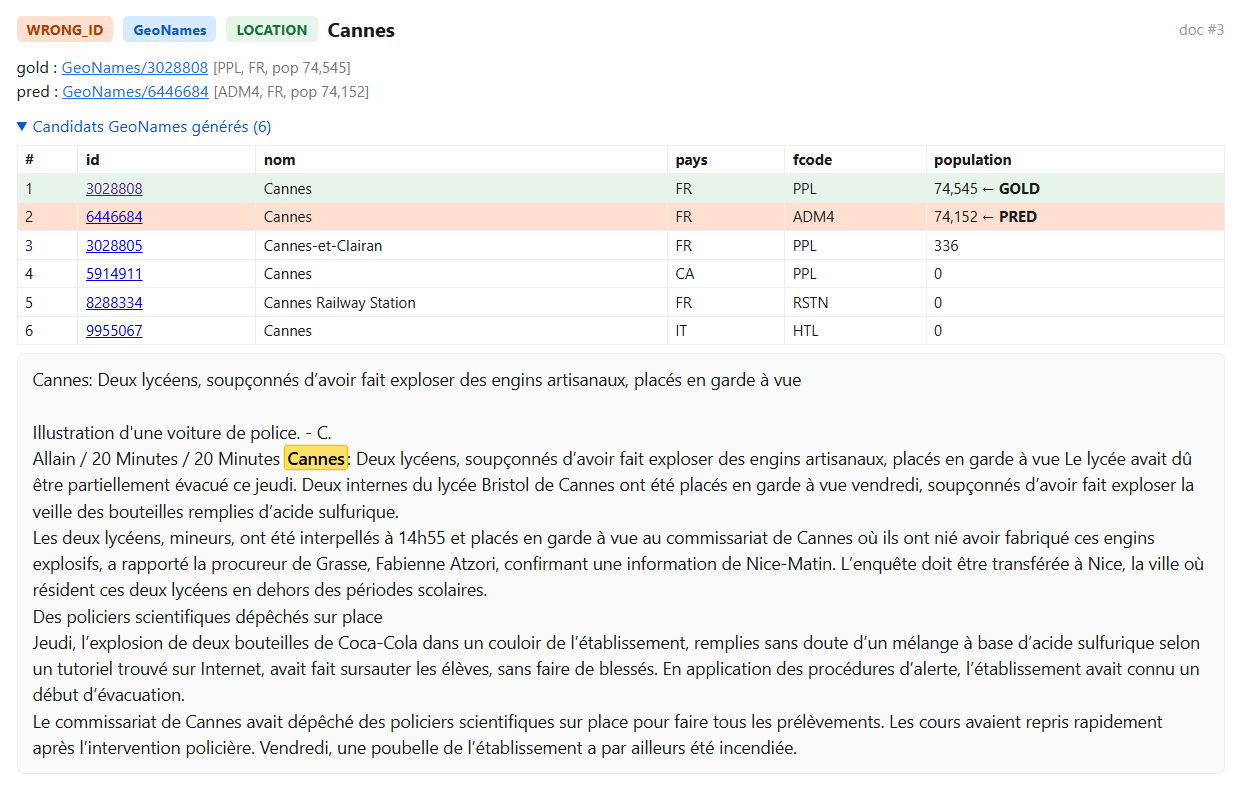
\includegraphics[width=\textwidth]{error_analysis_evallm.png}
\caption{Capture d'écran du visualiseur d'erreurs (cas « Cannes », doc~\#3). La référence
(Cannes \textsc{ppl}, id~3028808) figure dans la liste de candidats \emph{au rang~1}, mais le
post-traitement géographique a retenu la commune (\textsc{adm4}, id~6446684) à la place de la
localité.}
\label{fig:erreur}
\end{figure}

\begin{figure}[H]
\centering
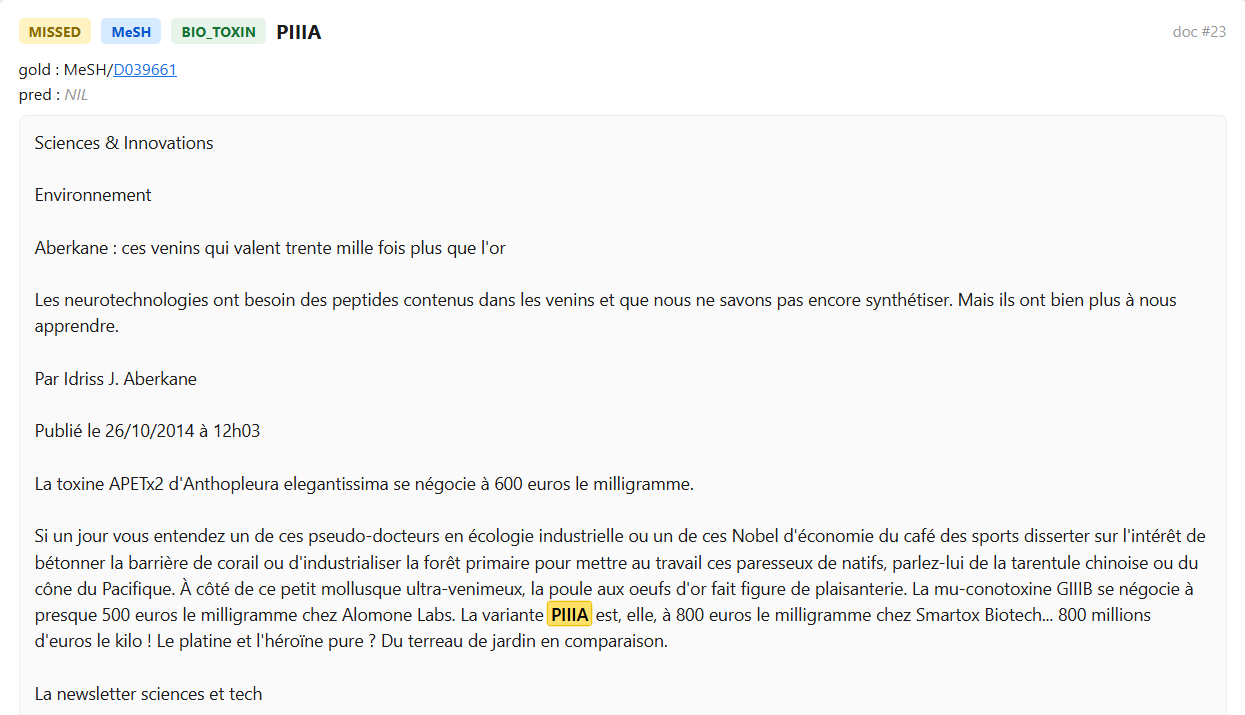
\includegraphics[width=\textwidth]{error_analysis_mesh_evallm.png}
\caption{Capture d'écran du visualiseur d'erreurs (cas « PIIIA », doc~\#23). La toxine « PIIIA »
(une conotoxine, type \textsc{bio\_toxin}) a pour référence MeSH~D039661, mais l'index ne lui
associe aucun candidat~: le système la laisse hors-référentiel (NIL) au lieu de la lier.}
\label{fig:erreur-mesh}
\end{figure}

\end{document}
